\documentclass[conference]{IEEEtran}
\usepackage{times}
\usepackage{graphicx}
% numbers option provides compact numerical references in the text.
\usepackage[numbers]{natbib}
\usepackage{multicol}
\usepackage[bookmarks=true]{hyperref}

\pdfinfo{
   /Author (Anonymous)
   /Title  (Extended Abstract: Grounding Language to Reward Functions with Abstract Markov Decision Processes)
   /CreationDate (D:20160503120000)
   /Subject (AMDPs, Robots, Language)
   /Keywords (Grounded Language; AMDP)
}

\begin{document}

% paper title
\title{Extended Abstract: Grounding Language to Reward Functions With Abstract Markov Decision Processes}

% You will get a Paper-ID when submitting a pdf file to the conference system
\author{%Author Names Omitted for Anonymous Review. Paper-ID [add your ID here]
\authorblockN{Dilip Arumugam}
\and
\authorblockN{Sidd Karamcheti}
\and
\authorblockN{James MacGlashan}
\and
\authorblockN{Nakul Gopalan}
\and
\authorblockN{Stefanie Tellex}
}

%\author{\authorblockN{Michael Shell}
%\authorblockA{School of Electrical and\\Computer Engineering\\
%Georgia Institute of Technology\\
%Atlanta, Georgia 30332--0250\\
%Email: mshell@ece.gatech.edu}
%\and
%\authorblockN{Homer Simpson}
%\authorblockA{Twentieth Century Fox\\
%Springfield, USA\\
%Email: homer@thesimpsons.com}
%\and
%\authorblockN{James Kirk\\ and Montgomery Scott}
%\authorblockA{Starfleet Academy\\
%San Francisco, California 96678-2391\\
%Telephone: (800) 555--1212\\
%Fax: (888) 555--1212}}


% avoiding spaces at the end of the author lines is not a problem with
% conference papers because we don't use \thanks or \IEEEmembership


% for over three affiliations, or if they all won't fit within the width
% of the page, use this alternative format:
%
%\author{\authorblockN{Michael Shell\authorrefmark{1},
%Homer Simpson\authorrefmark{2},
%James Kirk\authorrefmark{3},
%Montgomery Scott\authorrefmark{3} and
%Eldon Tyrell\authorrefmark{4}}
%\authorblockA{\authorrefmark{1}School of Electrical and Computer Engineering\\
%Georgia Institute of Technology,
%Atlanta, Georgia 30332--0250\\ Email: mshell@ece.gatech.edu}
%\authorblockA{\authorrefmark{2}Twentieth Century Fox, Springfield, USA\\
%Email: homer@thesimpsons.com}
%\authorblockA{\authorrefmark{3}Starfleet Academy, San Francisco, California 96678-2391\\
%Telephone: (800) 555--1212, Fax: (888) 555--1212}
%\authorblockA{\authorrefmark{4}Tyrell Inc., 123 Replicant Street, Los Angeles, California 90210--4321}}


\maketitle

\begin{abstract}
Deriving new methods of task decomposition has been central to the field of reinforcement learning. We examine a newly proposed method for hierarchical task decomposition known as abstract Markov decision processes (AMDPs) which maintains internal MDPs as natural layers of abstraction over some ``base'' input problem allowing for efficient planning. Inspired by prior work for grounding natural language to the reward function of a regular MDP, we consider the effect of grounding natural language with varying degrees of abstraction to the individual layers of abstraction within the AMDP. Hypothesizing that the accuracy of the grounding procedure would be greatest when the degree of abstraction between language and internal MDP match, we evaluate on all pairwise combinations. Our results, while proving our hypothesis to be incorrect, suggest that the AMDP framework has great potential for task decomposition as it captures logical relationships between layers of abstraction within the AMDP.
\end{abstract}

\IEEEpeerreviewmaketitle

\section{Introduction}
When dealing with the issue of efficiently solving large-scale sequential decision making problems defined by complex state-action spaces, the ability to identify and leverage multiple layers of abstraction is key. Developing good methods of abstraction represents a logical way to accelerate planning time by breaking apart large, complex tasks into smaller sub-tasks. Moreover, this notion of decomposing tasks into their smaller constituent pieces more closely resembles our own human methodology for solving problems by identifying and completing sub-goals. Our goal in this work is to analyze an alternative method of abstraction for sequential decision making problems that utilizes multiple layers of abstraction over all components of the Markov Decision Process (MDP) in order to efficiently learn in complex domains. In order to convey the strength of the abstraction imposed by the abstract Markov decision process (AMDP) formalism, we extend prior work on grounding natural language commands to reward functions and, in particular, evaluate the succeess of the grounding process as a measure of the strength of the abstraction.

\section{Prior Work}
Typically, methods of abstraction have been applied to only a single element of an MDP in the hopes of improving overall problem tractability. Specifically, there have been some approaches that attempt to perform state abstraction~\cite{Li2006TowardsAU} by compressing similar states into single units or intelligently pruning states that are irrelevant to the overall task from consideration. Other approaches examine abstraction over the action space via macro-actions~\cite{Hauskrecht1998HierarchicalSO} or options~\cite{Sutton1999BetweenMA} that compose sequences of atomic actions into a single ``larger'' or temporally extended action. Unfortunately, these methods suffer from potentially increasing the size of the state or action space thereby increasing the time needed for planning~\cite{Jong2008TheUO}.

\section{Abstract Markov Decision Processes}

Our approach in tackling this problem of abstraction is to utilize abstract Markov decision processes (AMDPs) which represent a decomposition of a regular MDP resulting in a tiered hierarchy where each level represents an abstraction over the previous one. To briefly summarize, MDPs are represented by a five-tuple: $\langle$ ${\cal S}$, ${\cal A}$, ${\cal T}$, ${\cal R}$, $\gamma$ $\rangle$, where ${\cal S}$ is the set of possible states in the world; ${\cal A}$ is a set of all available actions that can be executed; ${\cal T}$ is a function that computes the probability of transitioning from one state to another by executing an action; ${\cal R}$ is a function specifying the agent's reward for taking an action within a particular state ; and $\gamma$ is a discount factor.

Building on top of this, AMDPs take a layered approach by maintaining an internal stack of MDPs, each of which represents a different layer of abstraction over the input problem. The base (lowest) level MDP is always the MDP representing the original problem (i.e. the input MDP) while higher level MDPs are hard coded over smaller state and action spaces (with corresponding and distinct transition dynamics and reward functions). Each state and action in a higher level MDP is implemented as an abstraction over multiple states and actions in the lower level creating a many-to-one mapping (as we move up the stack) resulting in smaller, more tractable state-action spaces. Intuitively, moving up the stack of MDPs captures the notion of identifying smaller, easier sub-goals within the problem. 

In terms of execution, a learning agent always begins at the base level MDP; whenever an action must be selected at a lower level, the current state information is fed upward and mapped to the next highest level of the AMDP effectively forcing the agent to think at one higher level of abstraction. This process repeats until the top of the MDP stack is reached, at which point, standard reinforcement learning algorithms are applied in order to compute a stationary policy for the entire level (which is then stored and reused so as to avoid redundant computation). Given this policy, the action required at highest level of abstraction becomes known and is representative of a single sub-goal that need be solved in order to complete the overall task. A series of surjective state mappings are maintained from higher to lower level MDPs allowing for a sort of backpropagation to occur once the higher level sub-task has been identified. This process of mapping backwards, computing a policy, and taking the specified action then repeats all the way down back to the base level MDP at which the original high-level sub-goal is fully expanded into the set of lower level actions that represent the completion of the subgoal. It is important to note that since policies computed at each level of the AMDP are stored, the true cost of planning in an AMDP is only equivalent to the cost of planning and solving all higher level MDPs each of which is decreasing in size and complexity as we move up the AMDP stack.

\section{Evaluation}

\begin{figure}[tbp]
\begin{center}
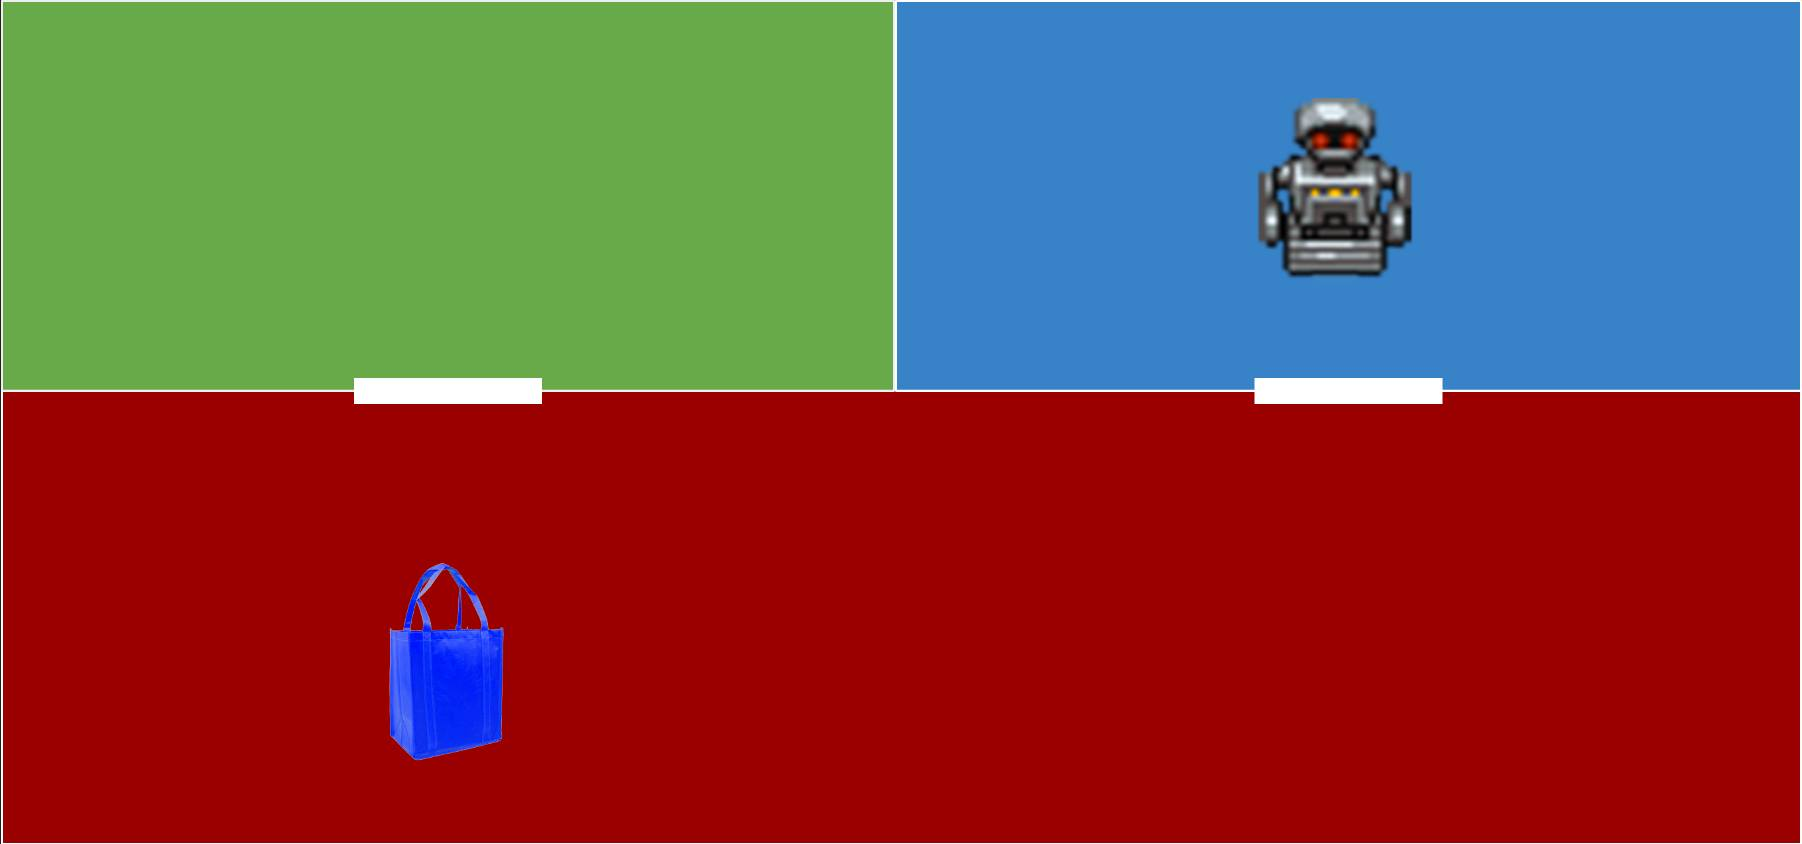
\includegraphics[scale=0.12]{images/cleanup}
\caption{\small An example of the CleanupWorld base level domain.
}
\end{center}
\end{figure}

\subsection{Experiments}

In order to examine the effectiveness of the abstractions imposed by the AMDP, we extend prior work on grounding natural language commands to the reward function of a Markov Decision Process (MDP). The primary contribution of this work is the ability to represent MDP reward functions as constrained conjunctions of propositional logic functions as well as combine learning from demonstration methods with language models to directly embed a user's verbal command into reward functions of the aforementioned form~\cite{MacGlashan2015GroundingEC}. Specifically, given a dataset of natural language commands and their associated task demonstrations, inverse reinforcement learning (IRL) is applied to the demonstrations in order to inform a distribution over possible reward functions which is then used to train a language model in a weakly supervised fashion. Following directly from the work of MacGlashan et. al., we use an IBM Model II Translation System for translating between natural language and reward functions (machine language), augmented by the probability of the provided demonstration under IRL. More specifically, we modify the IBM Model II decoding procedure to weight the probability of a given translation (the probability of a machine language command given the source language command) by the probability of the machine language command given the provided demonstration. With this process, the success of the resultant models in grounding reward function tasks is dependent on both the variety of natural language commands across the dataset as well as the strength of the IRL procedure over the provided demonstrations.

\subsection{Domain}

We show that grounding an arbitrary natural language command to a reward function will be most successful when the natural language command and reward function correspond to the same level of abstraction. Staying consistent with the experimental method used by MacGlashan et.al., we leverage objected-oriented MDPs~\cite{Diuk2008AnOR} within the Brown-UMBC Reinforcement Learning and Planning library (BURLAP) to conduct our experiments. For similar reasons, we also use the CleanupWorld domain inspired by Sokoban \cite{Junghanns2001SokobanEG}. In Figure 1, we provide an image of the standard CleanupWorld domain in a standard start configuration.
% INSERT FIGURE

We build our own AMDP over this domain with three \textbf{low}, \textbf{mid}, and \textbf{high} levels such that each level corresponds to a different level of task abstraction. The low-level MDP corresponds to simple directional commands, where the action space consists of moving one step in the north, south, east, or west direction. The mid-level MDP abstracts over the low-level MDP and encapsulates sub-goals which move the agent and blocks to specific doors and, subsequently, rooms. Finally, the high-level MDP abstracts away the notion of doors and contains the sub-goals of moving an agent or block to a particular room.

To test the effectiveness of using AMDPs, we collect datasets for each level, with each dataset consisting of a list of natural language commands that match the given level's abstraction and their respective demonstrations. The following are some examples of natural language commands at each level of the AMDP:

\begin{description}
\item[\textbf{Low:}] Go three steps south, then two steps east.
\item[\textbf{Mid:}] Go to the red door, then go into the red room.
\item[\textbf{High:}] Go to the green room.
\end{description}

Our experiment consists of training demonstration weighted IBM II Translation Models between every permutation of the levels of the AMDP. We then evaluate the models by passing in a natural language command of a given level into each of the three models. With this process, we hypothesized that the best results for a given level of the AMDP will match to natural language commands with of an identical degree of abstraction, rather than any others. We use Leave-One-Out (LOO) accuracy as the evaluation metric.

\subsection{Results}

The following table shows our LOO results for each swap. The rows are labeled with the level of the Natural Language (NLP) command, while the Columns designate the level of the MDP to which the language is grounded (the level-specific IBM II Translation system.)

\begin{table}[h!]
\centering
\caption{LOO Accuracy for each Swap}
\label{my-label}
\begin{tabular}{l|l|l|l|}
\cline{2-4}
                                  & MDP Level 0 & MDP Level 1 & MDP Level 2 \\ \hline
\multicolumn{1}{|l|}{NLP Level 0} & 36.7 \%      & 0.0\%       & \textbf{40.0\%}       \\ \hline
\multicolumn{1}{|l|}{NLP Level 1} & 10.7\%       & 3.57 \%     & 14.3\%       \\ \hline
\multicolumn{1}{|l|}{NLP Level 2} & \textbf{46.7\%}       & \textbf{26.7}\%       & 10.0\%       \\ \hline
\end{tabular}
\end{table}

Contrary to what we predicted, the grounding accuracies obtained when the levels of natural language and MDP match were not the most prominent at any layer of abstraction. Examining our results more closely, we find that there are some interesting properties of the abstraction that are captured in the results. Over the course of the subsequent error analysis, one universal problem present in our experiments is data sparsity; each experiment was conducted using only 30 samples (whereas the original experiments conducted by MacGlashan et.al. utilized more than 100 samples). 

We first notice that our worst result comes from using low-level language at the mid-level MDP; in the entire CleanupWorld AMDP, the jump in abstraction between levels is largest between the low and mid levels so the difficulty in grounding success when mixing between these levels is predictably difficult. Additionally, notice how low-level language commands like ``walk three steps south'' correspond to moving through a single door and entering a room (at the mid-level). Logically, it is harder to establish the translation between the given natural language and two, distinct actions; this fact becomes even more apparent when considering the accuracy when grounding low-level language to the high-level MDP. Since language commands like the previous example ground to a single ``move to rooom'' action in the high-level MDP, it makes sense that these groundings were successful. 

Returning to the notion of gap between layers of abstraction, we note that this gap is minimal between the mid and high levels of the AMDP which is reflected in our (relatively) high accuracies for both groundings involving these two levels exclusively. When examining the overall success of grounding in the low-level MDP, we recognize that the overall vocabulary of high-level commands is much smaller than that of low-level commands which, coupled with our data sparsity issues, make the IBM Model II translation more reliable at the higher level. We posit that the accuracy for low-level language groundings in the low-level MDP would be much higher provided a larger number of data samples.
\section{Conclusion and Future Work}
\label{sec:conclusion}

In this work, we analyzed AMDPs as a new, alternative framework for hierarchically decomposing large, intractable tasks into multiple layers with varying degress of abstraction. The goal of our analysis was to verify the strength and reliability of the proposed AMDP abstractions by examining the success of grounding natural language with varying degress of abstraction to reward functions in each layer of the AMDP. While our results do not support our initial hypothesis, it is clear that properties of the abstraction between layers of the AMDP are visible in the collected experimental results. Additionally, it is worth noting that all of our experiments were conducted using a very small amount of data in comparison to those of the original grounding reward functions work. We believe that more effort should be allocated towards data collection in order to definitively accept/reject our proposed hypothesis before continuing onwards to the more interesting and challenging problem of learning the layers of the AMDP given only the base-level MDP as input.


%% Use plainnat to work nicely with natbib.

\bibliographystyle{plainnat}
\bibliography{references}

\end{document}


